\documentclass{beamer}
\title{Terrain Discrimination}
\date{18. 12. 2019}
\author{Hanna Olbert, Lukas Kyzlik}

\usepackage[utf8]{inputenc}
\usepackage[IL2]{fontenc}
\usepackage[english]{babel}
\usepackage{amsmath,amsfonts,amssymb}

%\usepackage{a4wide}
\usepackage[shortlabels]{enumitem}
\usepackage{indentfirst}
%\usepackage{graphicx}
\usepackage{url}
\usepackage{textcomp}

\usetheme{Rochester}
\usecolortheme{seagull}

\addtobeamertemplate{navigation symbols}{}{%
    \usebeamerfont{footline}%
    \usebeamercolor[fg]{footline}%
    \hspace{1em}%
    \insertframenumber/\inserttotalframenumber
}

\begin{document}

%%%%%%
\frame{\titlepage}

%%%%%%%%%%%%%%%%%%%%%%%%%%%%%%%%%5
\section{Perceptron Classifier}
\frame{\sectionpage}

%%%%%%
\begin{frame}
\frametitle{Perceptron -- benchmark}

Perceptron(max\_iter=100000)

\begin{table}[]
\begin{tabular}{|l|l|}
\hline
Average training time [s] & 69.76 \\ \hline
Average score & 0.542 \\ \hline
\end{tabular}
\label{tab:perceptron}
\caption{Average results from 10 iterations of the test.}
\end{table}

\begin{block}{Conclusion}
  0.542 is benchmark we need to beat with more advanced methods to justify their use.
\end{block}
\end{frame}

%%%%%%%%%%%%%%%%%%%%%%%%%%%%%%%%%5
\section{Multy-Layer Perceptron (MLP) Classifier}
\frame{\sectionpage}

%%%%%%
\begin{frame}
\frametitle{MLP L-BFGS}
\textbf{Limited-memory BFGS} is optimization algorithm in the family of quasi-Newton methods. It should perform the best for small datasets like ours.
\\~\\
In the following tests we use this default values for MLP classifier (if some of them are changed, it is noted):
\begin{table}[h]
\begin{tabular}{|l|l|}
\hline
\textbf{Solver} & L-BFGS \\ \hline
\textbf{Alpha} & $10^{-5}$ \\ \hline
\textbf{Hidden layer sizes} & 1 layer, 15 neurons \\ \hline
\textbf{Random state} & fixed seed \\ \hline
\textbf{Activation function} & ReLU \\ \hline
\end{tabular}
\end{table}

\end{frame}

%%%%%%
\begin{frame}
\frametitle{MLP L-BFGS -- Activation functions}
\begin{figure}
\begin{centering}
  \includegraphics[scale=0.45]{mlp_activation_func.eps}
  \caption{Average results from 20 iterations with different activation functions.}
  \label{pic:activation_func}
\end{centering}
\end{figure}
\end{frame}

%%%%%%
\begin{frame}
\frametitle{MLP L-BFGS -- Activation functions}
\begin{block}{Conclusion}
  ReLU activation function gives the best results and is faster than most other functions for this problem.
\end{block}
\end{frame}

%%%%%%
\begin{frame}
\frametitle{MLP L-BFGS -- Number of neurons (1 hidden layer)}
\begin{figure}
\begin{centering}
  \includegraphics[scale=0.45]{mlp_1layer_neurons.eps}
  \caption{Average results from 50 iterations with different numbers of neurons in one hidden layer.}
  \label{pic:mlp_1layer_neurons}
\end{centering}
\end{figure}
\end{frame}

\begin{frame}
\frametitle{MLP L-BFGS -- Number of neurons (1 hidden layer)}
\begin{block}{Conclusion}
  Optimal number of neurons with one hidden layer from perspective accuracy is around 20 for this problem. However, it also has the longest training time. Higher numbers of neurons probably result in over-fitting.
\end{block}
\end{frame}

%%%%%%
\begin{frame}
\frametitle{MLP L-BFGS -- Number of neurons (2 hidden layes)}
\begin{figure}
\begin{centering}
  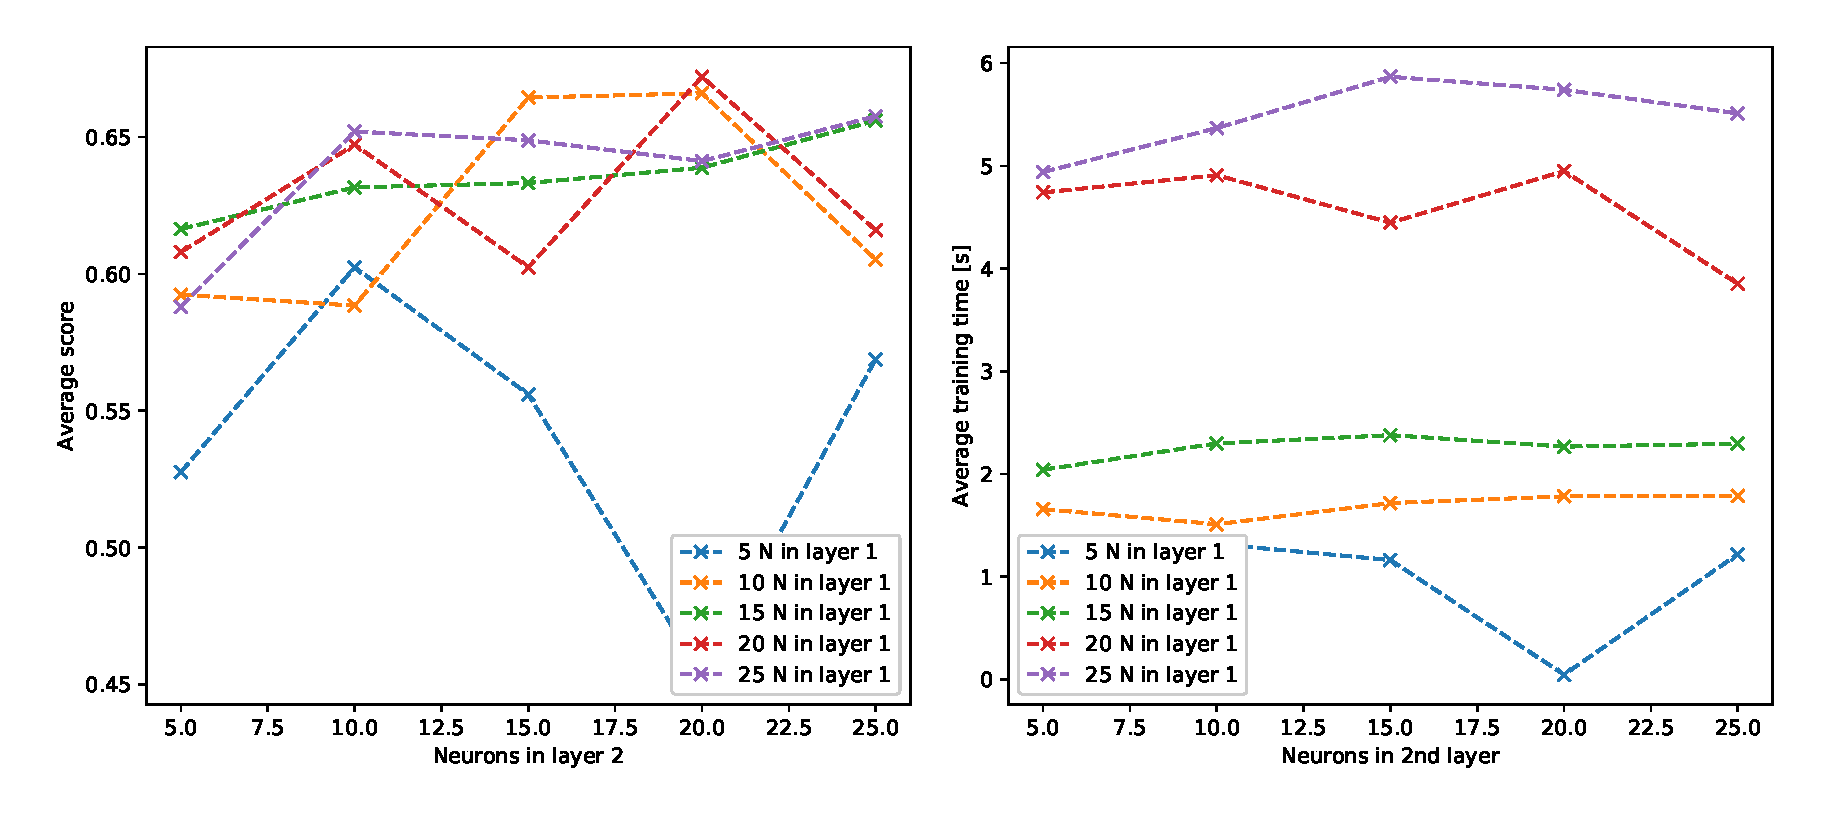
\includegraphics[scale=0.35]{mlp_2layer_neurons.eps}
  \caption{Average results from 50 iterations with different numbers of neurons in one hidden layer.}
  \label{pic:mlp_1layer_neurons}
\end{centering}
\end{figure}
\end{frame}


%%%%%%
\begin{frame}
\frametitle{MLP SGD}
\textbf{Stochastic gradient descent} is optimization algorithm for optimizing differentiable or subdifferentiable functions.
\\~\\
In the following tests we use this default values for MLP classifier (if some of them are changed, it is noted):
\begin{table}[h]
\begin{tabular}{|l|l|}
\hline
\textbf{Solver} & SGD \\ \hline
\textbf{Alpha} & $10^{-5}$ \\ \hline
\textbf{Hidden layer sizes} & 1 layer, 15 neurons \\ \hline
\textbf{Random state} & fixed seed \\ \hline
\textbf{Activation function} & ReLU \\ \hline
\textbf{Batch size} & 200 \\ \hline
\textbf{Initial learning rate} & 0.001 \\ \hline
\end{tabular}
\end{table}
\end{frame}

%%%%%%
\begin{frame}
\frametitle{MLP SGD -- Initial learning rate}
\begin{figure}
\begin{centering}
  \includegraphics[scale=0.48]{sgd_learning_rate.eps}
  \caption{Average results from 50 iterations with different initial learning rates.}
  \label{pic:learning_rate}
\end{centering}
\end{figure}
\end{frame}

%%%%%%
\begin{frame}
\frametitle{MLP SGD -- Batch size}
\begin{figure}
\begin{centering}
  \includegraphics[scale=0.45]{sgd_batch_size.eps}
  \caption{Average results from 20 iterations with different batch sizes.}
  \label{pic:batch_size}
\end{centering}
\end{figure}
\end{frame}

\begin{thebibliography}{9}

\bibitem{temp}


\end{thebibliography}

\end{document}
